\documentclass[eikonal.tex]{subfiles}

\begin{document}

\section{Background}\label{sec:background}

\begin{figure}[t]
  \centering
  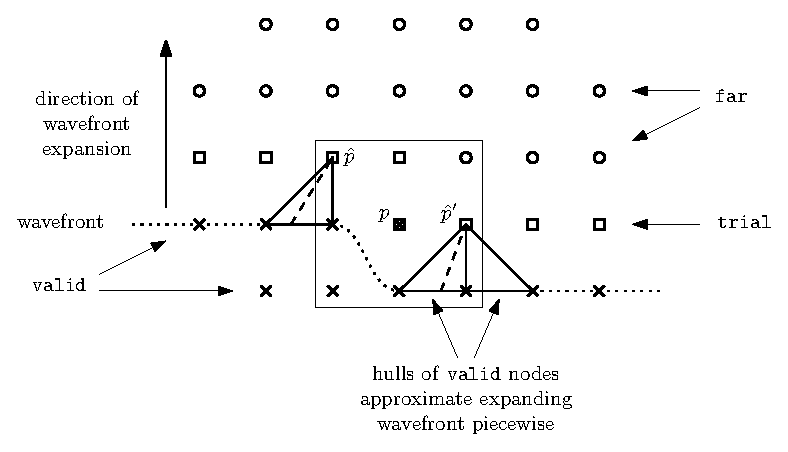
\includegraphics[width=0.9\linewidth]{overview.eps}
  \caption{An overview of a Dijkstra-like algorithm for solving the
    eikonal equation, \cref{eq:eikonal} (see
    \cref{alg:dijkstra-like}). The box surrounding $p$ depicts its
    neighborhood, \texttt{nb}$(p)$. Triangles represent updates. The
    dashed lines depict local rays: not necessarily the true
    minimizing rays.}
  \label{fig:overview}
\end{figure}

We now provide a brief overview of the eikonal equation and its
numerical solution on a regular grid. We then review the different
algorithms available for its solution, and sketch a generic
Dijkstra-like algorithm which we will refer to throughout the paper to
organize our results. Note that the FMM could be described by this
generic algorithm equally well. Since we focus on Dijkstra-like
algorithms here, our explanation of the fast sweeping and other
iterative methods will be brief.

\subsection{The eikonal equation}

With $n \geq 2$, and given a domain $\Omega \in \R^n$, the eikonal
equation is:
\begin{equation}\label{eq:eikonal}
  \norm{\nabla u(x)} = s(x), \qquad x \in \Omega,
\end{equation}
where $\|\cdot\|$ denotes the $\ell_2$ norm unless otherwise stated,
and $s : \Omega \to (0, \infty)$ is a fixed, positive \emph{slowness
  function}, which forms part of the problem data. Hence, we solve for
$u : \Omega \to \R_+$. The rest of the problem data is a subset
$D \subset \Omega$ where $u$ has been fixed; i.e.,
$\left. u \right|_D = g$ for some $g : D \to \R_+$. As an example, if
$s \equiv 1$ and $g \equiv 0$, then the solution of \cref{eq:eikonal}
is:
\begin{equation}
  \label{eq:distance-to-Omega}
  u(x) = d(x, D) = \min_{y \in D} \norm{x - y}.
\end{equation}
That is, $u$ is the distance to $D$ at each point in
$\Omega$. 

To numerically solve \cref{eq:eikonal}, first let
$\calG = \{p_i\} \subseteq \Omega$ be the set or grid of \emph{nodes}
where we would like to approximate the true solution $u$ with a
numerical solution $U : \calG \to \R_+$. Additionally, for each node
$p \in \calG$, define a set of neighbors,
$\neib(p) \subseteq \calG \backslash \set{p}$. Typically---for the FMM
and \texttt{olim6}, for instance---$\calG$ is taken to be a subset of
a lattice in $\R^n$ and $\neib(p)$ to be each node's $2n$ von Neumann
neighbors. With $\calG$ defined, we also define the set of
\emph{boundary nodes}, $\boundary \subseteq \calG$. It may happen that
the set $\boundary$ and $D$ do not coincide (e.g., $D$ could be a
curve which does not intersect $\calG$); to reconcile this difference,
the initial value of $U(p)$ for each $p \in \boundary$ must take
$g = \left. u \right|_D$ into account in the best way possible. This
problem has been approached in different ways, and is not the focus of
the present work~\cite{chopp2001some}.

Throughout, we make several simplifying assumptions.
\begin{itemize}
\item All boundary nodes coincide with grid points:
  $\boundary = D \subseteq \calG$.
\item The grid $\calG$ is a regular, uniform grid (a subset of a
  regular, uniform square lattice in 2D or cubic lattice in 3D). We
  denote grid nodes by $x \in \calG$.
\item When numerically computing a new value at a grid point
  $\hat{x} \in \calG$, we transform the neighborhood to the origin and
  scale the vertices so that they have integer values. The transformed
  update node is labeled $\hat{p}$. See \cref{ssec:notation} for a
  detailed explanation.
\end{itemize}

\subsection{Dijkstra-like algorithms}\label{ssec:dijkstra-like}
If we order nodes in $\mathcal{G}$ so that new solution values are
only ever computed using upwind nodes, the eikonal equation can be
solved directly; i.e., without the use of an iterative solver. To be
clear, this means that each new value of the solution is only ever
calculated using nodes that have smaller values. This is done using a
variant of Dijkstra's algorithm for finding shortest paths in a
network. Other algorithms which solve similar network flow problems
can also be used, but have different complexity
guarantees~\cite{chacon2012fast}. In particular, Dijkstra's algorithm
is a type of \emph{label-setting method} for finding shortest paths in
a network; there are also \emph{label-correcting
  methods}~\cite{bertsekas1998network}.

Using Dijkstra's algorithm to solve a ``continuous shortest path''
problem has been discovered in several contexts. The earliest such
development appears to be a theoretical result in computational
geometry due to Mitchell, Mount, and Papadimitriou, who used this idea
to compute exact polyhedral shortest paths (``discrete geodesics'') on
triangulated surfaces~\cite{mitchell1987discrete}. This was followed
by Tsitsiklis who developed a first-order semi-Lagrangian method for
solving isotropic optimal control problems on a uniform
grid~\cite{tsitsiklis1995efficient}. Finally, the fast marching
method, which uses a first-order upwind finite difference scheme was
developed by Sethian for isotropic front
propagation~\cite{sethian1996fast}. Many variations of these methods
have since been
developed~\cite{sethian2003ordered,kao2008legendre}. Our own
development resembles Tsitsisklis's, but extends it past its original
formulation.

To write down a generic Dijkstra-like algorithm, there are several
pieces of information which need to be kept track of. A data structure
we call \texttt{front} that stores an expanding wavefront is
maintained throughout the algorithm's execution. For each node $p$,
apart from the current value of $U(p)$, the most salient piece of
information is the \emph{state} of each node $p$, written
$p$\texttt{.state}
$\in \set{\texttt{valid}, \texttt{trial}, \texttt{far}}$. The meaning
of each of these states and each node's interaction with the
\texttt{front} data structure will become clear from the following
high-level description of the algorithm:

\begin{algorithm}
  \caption{A schematic Dijkstra-like algorithm for solving the eikonal
    equation.}\label{alg:dijkstra-like}
  \begin{enumerate}[nolistsep]
  \item For each $p \in \calG$, initially set $p$\texttt{.state} $=$
    \texttt{far} and $U(p) = \infty$.
  \item For each $p \in \boundary$, set $p$\texttt{.state} $=$
    \texttt{trial}, and set $U(p)$ to some user-defined initial value.
  \item While there are \texttt{trial} nodes left in $\calG$:
    \begin{enumerate}[nolistsep]
    \item Let $\pnew$ be the \texttt{trial} node in \texttt{front}
      with the smallest value $U(\pnew)$.\label{enum:get-node}
    \item Set $\pnew$\texttt{.state} $\gets$ \texttt{valid} and remove
      $\pnew$ from \texttt{front}.
    \item For each $\hat{p} \in \neib(\pnew)$, set
      $\hat{p}$\texttt{.state} $\gets$ \texttt{trial} if
      $\hat{p}$\texttt{.state} $=$ \texttt{far}.\label{enum:set-trial}
    \item For each $\hat{p} \in \neib(\pnew)$ such that
      $\hat{p}$\texttt{.state} $=$ \texttt{trial}, update
      $\hat{U} = U(\hat{p})$ and merge $\hat{p}$ into
      \texttt{front}.\label{enum:update-U}
    \end{enumerate}
  \end{enumerate}
\end{algorithm}

Specifying how \cref{enum:update-U} is to be performed is the crux of
developing a Dijkstra-like algorithm and is left intentionally
vague. This step involves indicating how nodes in $\neib(\hat{p})$ are
used to compute $\hat{U}$, and how they are organized into the
\texttt{front} data structure. The FMM uses an upwind finite
difference scheme where only \texttt{valid} nodes are used to compute
$\hat{U}$, and where nodes on the front are sorted using an
array-based heap implementing a priority
queue~\cite{sethian1996fast}. As an example, Tsitsiklis's algorithm
combines nodes in \texttt{valid} into sets whose convex hulls
approximate the surface of the expanding wavefront and then solves
local raytracing problems where rays emanate from these surfaces. The
method presented here operates in the same way (see
\cref{fig:overview}). For specific details, a general reference should
be consulted~\cite{sethian1999level}. In addition to
\cref{enum:update-U}, algorithm \cref{alg:dijkstra-like} is generic in
the following ways:
\begin{itemize}
\item As we mentioned before, there are different ways of computing
  $\boundary$ and subsequently approximating the initial value of $U$
  for $p \in \boundary$ using
  $g = \left. u \right|_D$~\cite{chopp2001some}
\item How we keep track of the node with the smallest value is
  variable: most frequently, as in Dijkstra's algorithm, a heap
  storing pointers to the nodes is used, leading to $O(N^n \log N)$
  update operations overall, where $N^n$ is the number of nodes. In
  fact, there are $O(N^n)$ variations using Dial's algorithm (a
  bucketed version of Dijkstra's algorithm), but these have not been
  used as extensively as Dijkstra-like
  algorithms~\cite{tsitsiklis1995efficient,kim2001calo,yatziv2006n}.
\item Related to the foregoing point, the arrangement of the nodes
  (into a grid or otherwise) varies; hence, the neighborhood of each
  node varies. This naturally affects the update procedure. A regular
  grid is simple to deal with, but Dijkstra-like methods have been
  extended to manifolds and unstructured meshes, where the situation
  is more
  involved~\cite{kimmel1998computing,sethian2000fast,bronstein2008numerical}.
\end{itemize}
Other problems can be solved using Dijkstra-like algorithms: the
static Hamilton-Jacobi equation, an anisotropic generalization of the
eikonal equation, can be solved using the ordered upwind
method~\cite{sethian2003ordered} and other recently introduced
methods~\cite{mirebeau2014efficient,mirebeau2014anisotropic}. Consequently,
the quasipotential of a nongradient stochastic differential equation
can be computed using the ordered line integral method, although the
considerations may be more
involved~\cite{dahiya2017ordered,dahiya2018ordered,yang2019computing}.

\subsection{Fast sweeping methods} Another approach to solving a
discretized version of \cref{eq:eikonal} is the fast sweeping
method~\cite{tsai2003fast,zhao2005fast}. Unlike Dijkstra-like methods,
which are direct solvers, the fast sweeping method is an iterative
solver using an upwind scheme and rotating cardinal sweep
directions. For problems where the characteristics of the solution
change direction infrequently, the algorithm obtains $O(N^n)$
complexity. A drawback of the method is that the asymptotic constant
for this complexity guarantee cannot be bound a priori and depends
heavily on the geometry of the problem. Fast sweeping methods have
been extended to Hamilton-Jacobi
equations~\cite{tsai2003fast,kao2008legendre}, and hybrid methods
combining the fast sweeping method with a Dijkstra-like method have
been introduced recently~\cite{chacon2012fast,chacon2015parallel}.

\end{document}

%%% Local Variables:
%%% mode: latex
%%% TeX-master: "sisc-eikonal.tex"
%%% End:
